\documentclass{article}

\usepackage[english]{babel}
\usepackage[utf8]{inputenc}
\usepackage{amsmath}
\usepackage{amsthm}
\usepackage{amssymb}
\usepackage{mathtools}
\usepackage{amsfonts}
\usepackage{subcaption}
\usepackage{graphicx}
\usepackage{wrapfig}
\usepackage{bbm}
\usepackage{dsfont}
\usepackage{listings}

% set up margin
\usepackage
[
  a4paper,
  left=3cm,
  right=3cm,
  top=3cm,
  bottom=3cm,
]
{geometry}

% set up header
\usepackage{fancyhdr}
\pagestyle{fancy}
\fancyhf{}
\lhead{6.438 Algorithms for Inference}
\chead{Problem Set 4}
\rhead{Hongzi Mao}
\cfoot{\thepage}
\rfoot{\footnotesize{\emph{Collaborated with: Hongzhou Ye, Zhiwei Ding}}}

% footer line
\renewcommand{\footrulewidth}{0.4pt}

% sans serif italic
\newcommand{\s}[1]{\textsf{\textit{#1}}}

% bold face sans serif
\newcommand{\bs}[1]{\textsf{\textbf{#1}}}

% set symbol
\usepackage[mathscr]{euscript}

% empty set
\let\emptyset\varnothing

% qed
\newcommand{\qeds}{\hfill\qedsymbol}

% math bold face
\newcommand{\bm}{\mathbf}

% argmax
\DeclareMathOperator*{\argmax}{argmax}
\DeclareMathOperator*{\argmin}{argmin}

% colorful reference
\usepackage{hyperref}
\usepackage{color}
\definecolor{darkred}{rgb}{0.7,0,0}
\definecolor{darkgreen}{rgb}{0,0.5,0}
\hypersetup{colorlinks=true,
        linkcolor=darkred,
        citecolor=darkgreen}
\urlstyle{same}

% independence symbol
\makeatletter
\newcommand*{\indep}{%
  \mathbin{%
    \mathpalette{\@indep}{}%
  }%
}
\newcommand*{\nindep}{%
  \mathbin{%                   % The final symbol is a binary math operator
    \mathpalette{\@indep}{\not}% \mathpalette helps for the adaptation
                               % of the symbol to the different math styles.
  }%
}
\newcommand*{\@indep}[2]{%
  \sbox0{$#1\perp\m@th$}%        box 0 contains \perp symbol
  \sbox2{$#1=$}%                 box 2 for the height of =
  \sbox4{$#1\vcenter{}$}%        box 4 for the height of the math axis
  \rlap{\copy0}%                 first \perp
  \dimen@=\dimexpr\ht2-\ht4-.2pt\relax
  \kern\dimen@
  {#2}
  \kern\dimen@
  \copy0 %                       second \perp
} 
\makeatother

%%%%%%%%%%%%%%%%%%%%%%%%%%%%%%%%%%%%%%%%%%%%%%%%%%%%%%%%%%%%%%%%%%%%%%%%
%%%%%%%%%%%%%%%%%%%%%%%%% Begin document here %%%%%%%%%%%%%%%%%%%%%%%%%%
%%%%%%%%%%%%%%%%%%%%%%%%%%%%%%%%%%%%%%%%%%%%%%%%%%%%%%%%%%%%%%%%%%%%%%%%
\begin{document}

\section*{Problem 5.1}
%
(a) We check local consistency by checking the marginals sum to 1 and the
edge marginals marginalize to node marginal. That is
%
\begin{align*}
	b_i(0) + b_i(1) = 0.5 + 0.5 = 1,
\end{align*}
%
for $\forall i \in \{1, 2, 3\}$; and
\begin{align*}
	b_{ij}(0,0) + b_{ij}(0,1) + b_{ij}(1,0) + b_{ij}(1,1) = 1,
\end{align*}
%
for $\forall i, j \in \{1, 2, 3\}, i \neq j$;
and\footnote{$b_i(1)$ checks out similarly for $\forall \{1,2,3\}$}
%
\begin{align*}
	b_{12}(0, 0) + b_{12}(0, 1) = 0.49 + 0.01 = 0.5 &= b_1(0),\\
	b_{12}(1, 0) + b_{12}(0, 0) = 0.01 + 0.49 = 0.5 &= b_2(0),\\
	b_{32}(0, 0) + b_{32}(0, 1) = 0.49 + 0.01 = 0.5 &= b_3(0),\\
	b_{32}(1, 0) + b_{32}(0, 0) = 0.01 + 0.49 = 0.5 &= b_2(0),\\
	b_{31}(0, 0) + b_{31}(0, 1) = 0.01 + 0.49 = 0.5 &= b_3(0),\\
	b_{31}(1, 0) + b_{31}(0, 0) = 0.49 + 0.01 = 0.5 &= b_1(0).\\
\end{align*} \qeds
%
\\

\noindent
(b) We prove this by contradiction. Suppose such distribution
$p_{\s{x}_1, \s{x}_2, \s{x}_3}(x_1, x_2, x_3)$ exists, then
\begin{align}
	&p_{\s{x}_1, \s{x}_2, \s{x}_3}(0, 0, 0) + p_{\s{x}_1, \s{x}_2, \s{x}_3}(0, 0, 1) = b_{12}(0, 0) = 0.49, \label{51b1}\\
	&p_{\s{x}_1, \s{x}_2, \s{x}_3}(0, 0, 0) + p_{\s{x}_1, \s{x}_2, \s{x}_3}(0, 1, 0) = b_{31}(0, 0) = 0.01, \label{51b2}\\
	&p_{\s{x}_1, \s{x}_2, \s{x}_3}(0, 0, 1) + p_{\s{x}_1, \s{x}_2, \s{x}_3}(1, 0, 1) = b_{32}(0, 1) = 0.01. \label{51b3}
\end{align}
%
Since we assume $p_{\s{x}_1, \s{x}_2, \s{x}_3}(\cdot)$ is a valid distribution, we have
\begin{align*}
	p_{\s{x}_1, \s{x}_2, \s{x}_3}(x_1, x_2, x_3) \geq 0,
\end{align*}
for $\forall (x_1, x_2, x_3) \in \{0, 1\}^3$.

Now, from Equation~\eqref{51b2}, we have
\begin{align*}
	p_{\s{x}_1, \s{x}_2, \s{x}_3}(0, 0, 0) \leq 0.01,
\end{align*}
from from Equation~\eqref{51b3}, we have
\begin{align*}
	p_{\s{x}_1, \s{x}_2, \s{x}_3}(0, 0, 1) \leq 0.01.
\end{align*}
%
Thus, 
\begin{align*}
	p_{\s{x}_1, \s{x}_2, \s{x}_3}(0, 0, 0) + p_{\s{x}_1, \s{x}_2, \s{x}_3}(0, 0, 1) \leq 0.01 + 0.01 = 0.02,
\end{align*}
%
which contradicts with Equation~\eqref{51b1}, where 
$p_{\s{x}_1, \s{x}_2, \s{x}_3}(0, 0, 0) + p_{\s{x}_1, \s{x}_2, \s{x}_3}(0, 0, 1) = 0.49$.
\qeds
\\
\\
\\
\\
\\
\\
\\
\\
\\
\\

\pagebreak
%
%%%%%%%%%%%%%%%%%%%%%%%%%%%%%%%%%%%%%%%%%%%%%%%%%%%%%%%%%%%%%%%%%%%%%%%% 
\section*{Problem 5.2}
(a) With slight abuse of notations, we index the node with the coordinate
$(i, j)$ in the image. Figure~\ref{f:52a} sketches the undirected graphs.
%
\begin{figure}[h]
  \centering
  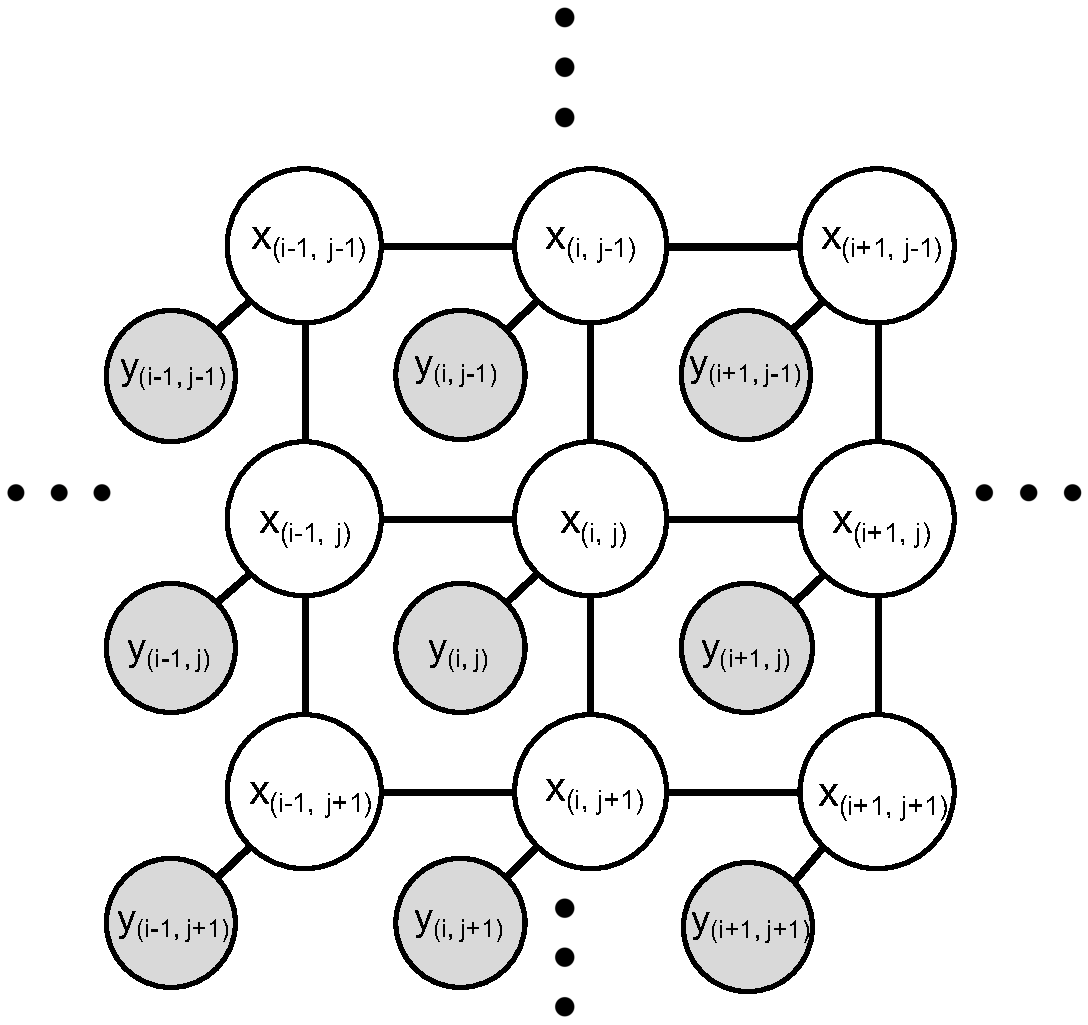
\includegraphics[width=0.4\columnwidth]{52a.pdf}
    \vspace{-0.1cm}
  \caption{Undirected graph of the 5.2 photography problem.}
  \label{f:52a}
\end{figure}
%

The potential function $\psi(x_i, y_i)$ is given by
\begin{align*}
	\psi(x_i, y_i) = \frac{1}{(2\pi)^{3/2}(\det {\bf\Lambda}_{x_i})^{1/2}}
	\exp\left[-\frac{1}{2}(y_i-\mu_{x_i})^T\mathbf{\Lambda}^{-1}_{x_i}(y_i - \mu_{x_i})\right] + \epsilon.
\end{align*}
\\

\noindent
(b) For the labeled masks, we empirically compute
\begin{align*}
	&\mu_\alpha = \frac{1}{N_\alpha}\sum_{i=1}^{N_\alpha}y_i,\\
	&\mathbf{\Lambda}_{\alpha} = \frac{1}{N_\alpha}\sum_{i=1}^{N_\alpha}\left[(y_i - \mu_\alpha)(y_i - \mu_\alpha)^T\right],
\end{align*}
where $N_\alpha$ is the number of pixels in the labeled mask.
%

In the \texttt{flower} example (raw $[0, 255]$ pixel representation), we have for the foreground
\begin{align*}
	\mu_1 = 
	\begin{bmatrix}
    168.29 \\
    95.19 \\
    8.48
\end{bmatrix}, \;\;\,
	\mathbf{\Lambda}_1 =
\begin{bmatrix}
 94.89 & 122.81 & 144.93 \\
 122.81 & 111.90 & 105.58 \\
 144.93 & 105.58 &  68.92
\end{bmatrix},
\end{align*}
and the background
\begin{align*}
	\mu_0 = 
	\begin{bmatrix}
    78.79 \\
    79.10 \\
    41.24
\end{bmatrix}, \;\;\,
	\mathbf{\Lambda}_0 =
\begin{bmatrix}
104.27 & 133.14 & 130.03 \\
133.14 & 106.70 & 121.70 \\
130.03 & 121.70 & 102.89
\end{bmatrix}.
\end{align*}
%

If we compute the mean and covariance using pixel range $[0, 1]$ instead of $[0, 255]$, we will have for the foreground
\begin{align*}
	\mu_1' = 
	\begin{bmatrix}
    0.6600 \\
    0.3733 \\
    0.0333
\end{bmatrix}, \;\;\,
	\mathbf{\Lambda}_1' =
\begin{bmatrix}
 0.4909 & 0.3091 & 0.0228 \\
 0.3091 & 0.2194 & 0.0133 \\
 0.0228 & 0.0133 & 0.0015
\end{bmatrix},
\end{align*}
and the background
\begin{align*}
	\mu_0' = 
	\begin{bmatrix}
    0.3090 \\
    0.3102 \\
    0.1617
\end{bmatrix}, \;\;\,
	\mathbf{\Lambda}_0' =
\begin{bmatrix}
0.1735 & 0.1665 & 0.0977 \\
0.1665 & 0.1639 & 0.0961 \\
0.0977 & 0.0961 & 0.0599
\end{bmatrix}.
\end{align*}

The code for this computation is attached in the bottom.
\\

\noindent
(c)
We denote the indices of the neighboring pixels of $j$ as $\partial j$. That is the observation $y_j$ is not a member of $\partial j$ and we consider the message from it separately. The update rule for the message passing is
\begin{align*}
	m_{j\to k}(x_k) &= \sum_{x_j} \psi_{jk}(x_j, x_k)\,\,m_{y_j\to x_j}(x_j) \prod_{l\in\partial{j}\backslash\{k\}}m_{l\to j}(x_j)\\
	&\propto \sum_{x_j} \big[0.9\times\mathds{1}_{x_j = x_k} + 0.1\times\mathds{1}_{x_j \neq x_k} \big] \times\\
	& \left\{\frac{1}{(2\pi)^{3/2}(\det {\bf\Lambda}_{x_j})^{1/2}} \exp\left[-\frac{1}{2}(y_j-\mu_{x_j})^T\mathbf{\Lambda}^{-1}_{x_j}(y_j - \mu_{x_j})\right] + \epsilon\right\}
	\times \prod_{l\in\partial{j}\backslash\{k\}}m_{l\to j}(x_j).
\end{align*}
%

To compute the marginal, the final belief update rule on $x_i$ is
\begin{align*}
	p_{\s{x}_i}(x_i) &\propto  m_{y_i\to x_i}(x_i) \prod_{j\in\partial{i}}m_{j\to i}(x_i)\\
	&\propto \left\{\frac{1}{(2\pi)^{3/2}(\det {\bf\Lambda}_{x_i})^{1/2}} \exp\left[-\frac{1}{2}(y_i-\mu_{x_i})^T\mathbf{\Lambda}^{-1}_{x_i}(y_i - \mu_{x_i})\right] + \epsilon\right\}
	\times \prod_{j\in\partial{i}}m_{j\to i}(x_i).
\end{align*}
\\

\noindent
(d) We visualize the pixel marginals in Figure~\ref{f:52d}.
%
The ``weak'' beliefs are the pixels with grey colors. That is, the underlining
marginals spreads the probability mass between foreground and background.
%
In early iterations (e.g., iteration 1 and 2), there are a few black-grey dots inside
the flower foreground regions. These pixels in the original graph looks a bit green-ish,
which leads to a large probability value in the observation-pixel edge Gaussian
distribution. Over time, the neighboring pixels will overcome this belief and ``absorb''
those grey dots by foreground belief in white.
%

The loopy BP first converges the clear values---red flowers in the foreground, with mean 
close to the empirical foreground mean, and the object clusters close each other; green 
grass in the background for similar reasons. There are an green ``island'' in the left
flower that is difficult to converge to the foreground. The reason is that it has a
significant size of green inside the flower red, which self-reinforce its background
position inside the foreground region.
%
\begin{figure*}[t]
\captionsetup[subfigure]{labelformat=empty}
\centering
%
\begin{subfigure}[t]{0.19\textwidth}
\centering

\includegraphics[width=\textwidth]{./images/marginals_iter_1.png}
\vspace{-0.6cm}
\caption{iteration=1}
\end{subfigure}
\begin{subfigure}[t]{0.19\textwidth}
\centering

\includegraphics[width=\textwidth]{./images/marginals_iter_2.png}
\vspace{-0.6cm}
\caption{iteration=2}
\end{subfigure}
\begin{subfigure}[t]{0.19\textwidth}
\centering

\includegraphics[width=\textwidth]{./images/marginals_iter_3.png}
\vspace{-0.6cm}
\caption{iteration=3}
\end{subfigure}
\begin{subfigure}[t]{0.19\textwidth}
\centering

\includegraphics[width=\textwidth]{./images/marginals_iter_4.png}
\vspace{-0.6cm}
\caption{iteration=4}
\end{subfigure}
\begin{subfigure}[t]{0.19\textwidth}
\centering

\includegraphics[width=\textwidth]{./images/marginals_iter_5.png}
\vspace{-0.6cm}
\caption{iteration=5}
\end{subfigure}
\begin{subfigure}[t]{0.19\textwidth}
\centering

\includegraphics[width=\textwidth]{./images/marginals_iter_6.png}
\vspace{-0.6cm}
\caption{iteration=6}
\end{subfigure}
\begin{subfigure}[t]{0.19\textwidth}
\centering

\includegraphics[width=\textwidth]{./images/marginals_iter_7.png}
\vspace{-0.6cm}
\caption{iteration=7}
\end{subfigure}
\begin{subfigure}[t]{0.19\textwidth}
\centering

\includegraphics[width=\textwidth]{./images/marginals_iter_8.png}
\vspace{-0.6cm}
\caption{iteration=8}
\end{subfigure}
\begin{subfigure}[t]{0.19\textwidth}
\centering

\includegraphics[width=\textwidth]{./images/marginals_iter_9.png}
\vspace{-0.6cm}
\caption{iteration=9}
\end{subfigure}
\begin{subfigure}[t]{0.19\textwidth}
\centering

\includegraphics[width=\textwidth]{./images/marginals_iter_10.png}
\vspace{-0.6cm}
\caption{iteration=10}
\end{subfigure}
\begin{subfigure}[t]{0.19\textwidth}
\centering

\includegraphics[width=\textwidth]{./images/marginals_iter_11.png}
\vspace{-0.6cm}
\caption{iteration=11}
\end{subfigure}
\begin{subfigure}[t]{0.19\textwidth}
\centering

\includegraphics[width=\textwidth]{./images/marginals_iter_12.png}
\vspace{-0.6cm}
\caption{iteration=12}
\end{subfigure}
\begin{subfigure}[t]{0.19\textwidth}
\centering

\includegraphics[width=\textwidth]{./images/marginals_iter_13.png}
\vspace{-0.6cm}
\caption{iteration=13}
\end{subfigure}
\begin{subfigure}[t]{0.19\textwidth}
\centering

\includegraphics[width=\textwidth]{./images/marginals_iter_14.png}
\vspace{-0.6cm}
\caption{iteration=14}
\end{subfigure}
\begin{subfigure}[t]{0.19\textwidth}
\centering

\includegraphics[width=\textwidth]{./images/marginals_iter_15.png}
\vspace{-0.6cm}
\caption{iteration=15}
\end{subfigure}
\begin{subfigure}[t]{0.19\textwidth}
\centering

\includegraphics[width=\textwidth]{./images/marginals_iter_16.png}
\vspace{-0.6cm}
\caption{iteration=16}
\end{subfigure}
\begin{subfigure}[t]{0.19\textwidth}
\centering

\includegraphics[width=\textwidth]{./images/marginals_iter_17.png}
\vspace{-0.6cm}
\caption{iteration=17}
\end{subfigure}
\begin{subfigure}[t]{0.19\textwidth}
\centering

\includegraphics[width=\textwidth]{./images/marginals_iter_18.png}
\vspace{-0.6cm}
\caption{iteration=18}
\end{subfigure}
\begin{subfigure}[t]{0.19\textwidth}
\centering

\includegraphics[width=\textwidth]{./images/marginals_iter_19.png}
\vspace{-0.6cm}
\caption{iteration=19}
\end{subfigure}
\begin{subfigure}[t]{0.19\textwidth}
\centering

\includegraphics[width=\textwidth]{./images/marginals_iter_20.png}
\vspace{-0.6cm}
\caption{iteration=20}
\end{subfigure}
\begin{subfigure}[t]{0.19\textwidth}
\centering

\includegraphics[width=\textwidth]{./images/marginals_iter_21.png}
\vspace{-0.6cm}
\caption{iteration=21}
\end{subfigure}
\begin{subfigure}[t]{0.19\textwidth}
\centering

\includegraphics[width=\textwidth]{./images/marginals_iter_22.png}
\vspace{-0.6cm}
\caption{iteration=22}
\end{subfigure}
\begin{subfigure}[t]{0.19\textwidth}
\centering

\includegraphics[width=\textwidth]{./images/marginals_iter_23.png}
\vspace{-0.6cm}
\caption{iteration=23}
\end{subfigure}
\begin{subfigure}[t]{0.19\textwidth}
\centering

\includegraphics[width=\textwidth]{./images/marginals_iter_24.png}
\vspace{-0.6cm}
\caption{iteration=24}
\end{subfigure}
\begin{subfigure}[t]{0.19\textwidth}
\centering

\includegraphics[width=\textwidth]{./images/marginals_iter_25.png}
\vspace{-0.6cm}
\caption{iteration=25}
\end{subfigure}
\begin{subfigure}[t]{0.19\textwidth}
\centering

\includegraphics[width=\textwidth]{./images/marginals_iter_26.png}
\vspace{-0.6cm}
\caption{iteration=26}
\end{subfigure}
\begin{subfigure}[t]{0.19\textwidth}
\centering

\includegraphics[width=\textwidth]{./images/marginals_iter_27.png}
\vspace{-0.6cm}
\caption{iteration=27}
\end{subfigure}
\begin{subfigure}[t]{0.19\textwidth}
\centering

\includegraphics[width=\textwidth]{./images/marginals_iter_28.png}
\vspace{-0.6cm}
\caption{iteration=28}
\end{subfigure}
\begin{subfigure}[t]{0.19\textwidth}
\centering

\includegraphics[width=\textwidth]{./images/marginals_iter_29.png}
\vspace{-0.6cm}
\caption{iteration=29}
\end{subfigure}
\begin{subfigure}[t]{0.19\textwidth}
\centering

\includegraphics[width=\textwidth]{./images/marginals_iter_30.png}
\vspace{-0.6cm}
\caption{iteration=30}
\end{subfigure}

%
\caption{Visualizing the expectation in pixel marginals. The foreground is indicated by white.}
\label{f:52d}
\end{figure*}

\pagebreak
The code for this problem is
\lstset{language=Python}
\lstset{frame=lines}
\lstset{caption={Using parallel sum product algorithm for separating
image foreground and background}}
\lstset{label={code:photography}}
\lstset{basicstyle=\footnotesize}
\begin{lstlisting}
import numpy as np
from scipy import misc
from bp import belief_propagation
from mean_var import compute_mean_var


def normalize_img(img):
    normalized_img = np.zeros(img.shape)
    for i in range(img.shape[0]):
        for j in range(img.shape[1]):
            for k in range(3):
                normalized_img[i, j, k] = float(img[i, j, k]) / 255.0
    return normalized_img


def visualize_marginals(img, marginals, file_name):
    array = np.zeros([img.shape[0], img.shape[1]])
    for (i, j) in marginals:
        array[i, j] = marginals[(i, j)][0]
    array = 1 - array  # revert black & white
    array *= 255
    misc.imsave(file_name, array)


def main():
    image_file = './images/flower.bmp'
    foreground_file = './images/foreground.bmp'
    background_file = './images/background.bmp'

    image = misc.imread(image_file, flatten= 0)
    image = normalize_img(image)  # between [0, 1]
    foreground = misc.imread(foreground_file, flatten= 0)
    background = misc.imread(background_file, flatten= 0)

    mean_foreground, var_foreground = \
        compute_mean_var(image, foreground)

    mean_background, var_background = \
        compute_mean_var(image, background)

    mean_foreground = mean_foreground.reshape(-1, 1)
    mean_background = mean_background.reshape(-1, 1)

    det_foreground = np.linalg.det(var_foreground)
    det_background = np.linalg.det(var_background)

    inv_foreground = np.linalg.inv(var_foreground)
    inv_background = np.linalg.inv(var_background)

    eps = 0.01

    # neighbor pixel edge potentials
    psi_neighbors = {}
    psi_neighbors[(0, 0)] = 0.9
    psi_neighbors[(1, 1)] = 0.9
    psi_neighbors[(0, 1)] = 0.1
    psi_neighbors[(1, 0)] = 0.1

    # fill in the potential functions
    node_potential = {}
    edge_potential = {}

    for i in range(image.shape[0]):
        for j in range(image.shape[1]):
            # node potential is influenced by the observation
            img_vec = image[i,j].reshape(-1, 1)
            node = {}
            node[1] = 1 / ((2 * np.pi) ** (3/2) * det_foreground ** (1/2)) * \
                np.exp(-0.5 * ((img_vec - mean_foreground).T.dot(inv_foreground)).dot(
                (img_vec - mean_foreground))) + eps
            node[0] = 1 / ((2 * np.pi) ** (3/2) * det_background ** (1/2)) * \
                np.exp(-0.5 * ((img_vec - mean_background).T.dot(inv_background)).dot(
                (img_vec - mean_background))) + eps
            node_potential[(i, j)] = node
            # edge potential among the pixels
            if i - 1 >= 0:
                if ((i - 1, j), (i, j)) not in edge_potential:
                    edge_potential[((i, j), (i - 1, j))] = psi_neighbors
            if i + 1 < image.shape[0]:
                if ((i + 1, j), (i, j)) not in edge_potential:
                    edge_potential[((i, j), (i + 1, j))] = psi_neighbors
            if j - 1 >= 0:
                if ((i, j - 1), (i, j)) not in edge_potential:
                    edge_potential[((i, j), (i, j - 1))] = psi_neighbors
            if j + 1 < image.shape[1]:
                if ((i, j + 1), (i, j)) not in edge_potential:
                    edge_potential[((i, j), (i, j + 1))] = psi_neighbors

    # get marginal at every step
    d = 0
    for marginals in belief_propagation(node_potential, edge_potential, 30):
        d += 1
        visualize_marginals(image, marginals,
            './images/marginals_iter_' + str(d) + '.png')
        print('Step', d)


if __name__ == '__main__':
    main()
\end{lstlisting}

The library code \texttt{bp.py} (inherited from pset 3) is
\lstset{language=Python}
\lstset{frame=lines}
\lstset{caption={bp.py}}
\lstset{label={code:bp}}
\lstset{basicstyle=\footnotesize}
\begin{lstlisting}
import numpy as np


def ep(edge_potential, i, j, var_i, var_j):
    if (i, j) in edge_potential:
        return edge_potential[(i, j)][var_i, var_j]
    elif (j, i) in edge_potential:
        return edge_potential[(j, i)][var_j, var_i]
    else:
        return None


def get_msg(i, j, node_potential, edge_potential, messages, neighbors, normalize=True):
    # get msg_{i->j}(var)
    distant_msg = {0: 1, 1: 1}
    for k in neighbors[i]:
        if k != j:
            distant_msg[0] *= messages[(k, i)][0]
            distant_msg[1] *= messages[(k, i)][1]

    msg = {}
    msg[0] = node_potential[i][0] * ep(edge_potential, i, j, 0, 0) * distant_msg[0] \
           + node_potential[i][1] * ep(edge_potential, i, j, 1, 0) * distant_msg[1]
    msg[1] = node_potential[i][0] * ep(edge_potential, i, j, 0, 1) * distant_msg[0] \
           + node_potential[i][1] * ep(edge_potential, i, j, 1, 1) * distant_msg[1]

    if normalize:
        s = msg[0] + msg[1]
        msg[0] /= s
        msg[1] /= s

    return msg


def normalize_marginals(marginals):
    for node in marginals:
        p_sum = marginals[node][0] + marginals[node][1]
        marginals[node][0] /= p_sum
        marginals[node][1] /= p_sum


def belief_propagation(node_potential, edge_potential, diameter=np.inf):
    '''
    node_potential: {i -> node_potential}
    edge_potential: {(i, j) -> edge_potential}
    output: {i -> marginal}
    '''
    
    # find neighbor nodes for each node
    neighbors = {}
    for i in node_potential:
        neighbors[i] = set()
    for (i, j) in edge_potential:
        neighbors[i].add(j)
        neighbors[j].add(i)

    # initialize random message
    messages = {}
    init_msg = {0: 1, 1: 1}
    for (i, j) in edge_potential:
        messages[(i, j)] = init_msg
        messages[(j, i)] = init_msg

    diam = min(diameter, len(node_potential))

    # tree diameter <= total number of nodes
    for _ in range(diam):
        new_messages = {}
        for i in node_potential:
            for j in neighbors[i]:
                msg = get_msg(
                    i, j,
                    node_potential,
                    edge_potential,
                    messages,
                    neighbors)
                new_messages[(i, j)] = msg
        assert len(new_messages) == len(messages)
        messages = new_messages

        # compute marginals
        marginals = {}
        for i in node_potential:
            marginals[i] = {}
            msg = {0: 1, 1: 1}
            for j in neighbors[i]:
                msg[0] *= messages[(j, i)][0]
                msg[1] *= messages[(j, i)][1]
            marginals[i][0] = node_potential[i][0] * msg[0]
            marginals[i][1] = node_potential[i][1] * msg[1]

        # normalize marginals
        normalize_marginals(marginals)

        yield marginals

\end{lstlisting}

The axillary code for computing empirical mean and covariance is 
\lstset{language=Python}
\lstset{frame=lines}
\lstset{caption={mean\_var.py}}
\lstset{label={code:bp}}
\lstset{basicstyle=\footnotesize}
\begin{lstlisting}
import numpy as np
from scipy import misc


def compute_mean_var(image, ground):
    num_pixels = 0
    mean = np.zeros(3)
    sum_val = np.zeros(3)

    assert image.shape[0] == ground.shape[0]
    assert image.shape[1] == ground.shape[1]

    for i in range(image.shape[0]):
        for j in range(image.shape[1]):
            if ground[i, j] == 1:
                sum_val += image[i, j]
                num_pixels += 1

    if num_pixels > 0:
        mean = sum_val / num_pixels

    var = np.zeros([3, 3])
    sum_val = np.zeros([3, 3])

    for i in range(image.shape[0]):
        for j in range(image.shape[1]):
            if ground[i, j] == 1:
                val = image[i, j].reshape(-1, 1)
                sum_val += val.dot(val.T)

    if num_pixels > 0:
        var = sum_val / num_pixels

    return mean, var

\end{lstlisting}
\pagebreak

%%%%%%%%%%%%%%%%%%%%%%%%%%%%%%%%%%%%%%%%%%%%%%%%%%%%%%%%%%%%%%%%%%%%%%%% 
\section*{Problem 5.3}
\end{document}